\documentclass{beamer}

%%%%%%%%%%%%%%%%%%%%%%%%%%%%%%%%%%%%%%%%%%%%%%%%%%%%%%%%%%%%%%%%%%%%%%%
% Definicion de paquetes
\usepackage{minted}
\usepackage[utf8]{inputenc}
\usepackage[spanish]{babel}
\usepackage{hyperref}
\usepackage[nodayofweek,level]{datetime}
\usepackage{xargs}
\usepackage[colorinlistoftodos,prependcaption,textsize=tiny]{todonotes}
\presetkeys{todonotes}{inline}{}
\usepackage{pgfpages}

%%%%%%%%%%%%%%%%%%%%%%%%%%%%%%%%%%%%%%%%%%%%%%%%%%%%%%%%%%%%%%%%%%%%%%%
% Definición de comandos
\setlength{\marginparwidth}{2cm}
% \unsure{I'm not sure}
\newcommandx{\unsure}[2][1=]{\todo[linecolor=red,backgroundcolor=red!25,bordercolor=red,#1]{#2}}
% \change{This must be changed}
\newcommandx{\change}[2][1=]{\todo[linecolor=blue,backgroundcolor=blue!25,bordercolor=blue,#1]{#2}}
% \info{Just information}
\newcommandx{\info}[2][1=]{\todo[linecolor=green,backgroundcolor=green!25,bordercolor=green,#1]{#2}}
% \improvement{THIS must be improved}
\newcommandx{\improvement}[2][1=]{\todo[linecolor=orange,backgroundcolor=orange!25,bordercolor=orange,#1]{#2}}
\newcommandx{\thiswillnotshow}[2][1=]{\todo[disable,#1]{#2}}
\newcommand{\mydate}{\formatdate{15}{12}{2021}}

\graphicspath{ {images/} }

%%%%%%%%%%%%%%%%%%%%%%%%%%%%%%%%%%%%%%%%%%%%%%%%%%%%%%%%%%%%%%%%%%%%%%%
% Beamer
\usetheme{Madrid}
\AtBeginEnvironment{minted}{\fontsize{12}{12}\selectfont}
% \setbeameroption{show notes on second screen=right}
% \setbeameroption{show only notes}
% \setbeameroption{show notes}
% \setbeamertemplate{note page}[default]
\setbeamertemplate{caption}{\raggedright\insertcaption\par}
%%%%%%%%%%%%%%%%%%%%%%%%%%%%%%%%%%%%%%%%%%%%%%%%%%%%%%%%%%%%%%%%%%%%%%%
% Título
\title[CAP]{Paso de mensajes con Erlang}
\author[M. Ruiz (UCM)]{Miguel Emilio Ruiz Nieto}
\date{\mydate}
%%%%%%%%%%%%%%%%%%%%%%%%%%%%%%%%%%%%%%%%%%%%%%%%%%%%%%%%%%%%%%%%%%%%%%%
%% Empieza el documento
\begin{document}
  \begin{frame}
    \titlepage
  \end{frame}

  \begin{frame}{Contenidos}
    \tableofcontents[hideallsubsections]
  \end{frame}

  \section{Introducción}
  \begin{frame}{Introducción}
    \begin{itemize}
      \item Hemos visto cómo funciona en computación distribuida el paso de
      mensajes qué problemas puede resolver
      \item Ahora nos centraremos en cómo funciona el paso de mensajes en Erlang
      y sus aplicaciones
    \end{itemize}
  \end{frame}

  \section{Erlang}
    \subsection{Historia}
      \begin{frame}{Erlang}
        \begin{itemize}
          \item Lenguaje de programación desarrollado en Ericsson
          \item Orientado a sistemas distribuidos:
          \begin{itemize}
            \item Modelo de actores
            \item Paso de mensajes
            \item Tolerancia a fallos
            \item Alta disponibilidad
            \item Filosofía ``Let it crash''
          \end{itemize}
        \end{itemize}
      \end{frame}

      \subsection{Sintaxis}
      \begin{frame}[fragile]{Erlang. Sintaxis}
        \begin{minted}{erlang}
          % Proceso se envia mensaje así mismo
          1> Pid = self().
          <0.84.0>
          2> Pid ! hello.
          hello
        \end{minted}
      \end{frame}

      \begin{frame}[fragile]{Erlang. Sintaxis}
        \begin{minted}{erlang}
          % Crear un nuevo proceso
          Pid = spawn(fun() -> ok end).
          <0.86.0>
          2> Pid ! hello .
          hello
        \end{minted}
      \end{frame}

      \begin{frame}[fragile]{Erlang. Sintaxis}
        \begin{minted}{erlang}
          loop(State) ->
            receive
              Pattern1 when Guard1 -> Expr1;
              Pattern2 when Guard2 -> Expr2;
              Pattern3 -> Expr3
            end.
        \end{minted}
      \end{frame}

      \begin{frame}
        \begin{figure}
          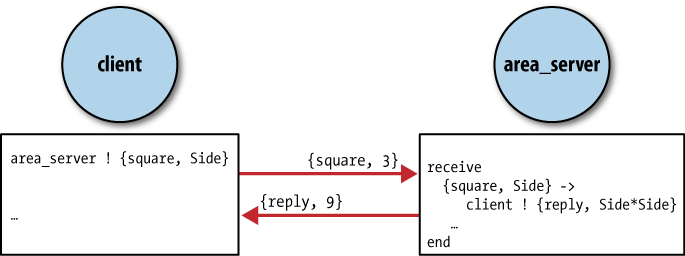
\includegraphics{actor-modelling.png}
        \end{figure}
      \end{frame}

      \begin{frame}{Erlang. Paso de mensajes}
        \begin{figure}
          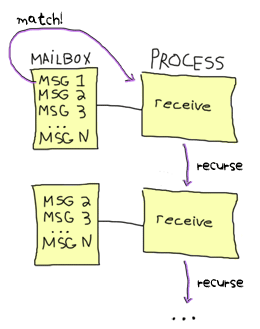
\includegraphics[width=0.5\textwidth]{msg-match.png}
        \end{figure}
      \end{frame}

  \section{Ejemplo práctico}
    \begin{frame}{Ejemplo práctico}
      \todo{usar el ejemplo del banco}
    \end{frame}

    \begin{frame}{Notas}
      \begin{itemize}
        \item Este ejemplo es la manera más ``explícita'' de implementar
        un servidor con estado
        \item Existen \textit{behaviors} dentro del lenguaje para construir
        este tipo de arquitecturas
      \end{itemize}
    \end{frame}

  \section{Conclusiones}
    \begin{frame}{Conclusiones}
      \begin{itemize}
        \item Erlang y MPI no resuelven los mismos problemas
        \item Implementar un
        \item c
      \end{itemize}
    \end{frame}

  \section{Bibliografía}
    \begin{frame}{Bibliografía}
      \begin{itemize}
        \item Getting Started with Erlang \url{https://www.erlang.org/doc/getting_started/intro.html}
        \item Learn You Some Erlang for Great Good! \url{https://learnyousomeerlang.com}
      \end{itemize}
    \end{frame}
\end{document}
